\begin{wrapfigure}[0]{r}{0pt}
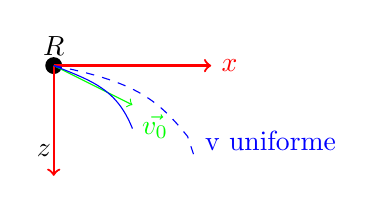
\begin{tikzpicture}
	\draw[fill=black] (0, 0) circle (0.1) node [above] {$R$};
	\draw[->, red, thick] (0, 0) -- (2, 0) node [right] {$x$};
	\draw[->, red, thick] (0, 0) -- (0, -1.4);
	\node[red, left, label=$z$] at (0, -1.4) {};
	\draw[->, green] (0, 0) -- (1, -0.5) node [below right] {$\vec{v_0}$};
	\draw[blue, thin] (0, 0) .. controls (0.5, -0.2) and (0.8, -0.3) .. (1, -0.8);
\draw[blue, dashed, thin] (0, 0) .. controls (1, -0.2) and (1.3, -0.4) .. (1.7, -0.9) -- (1.8, -1.2) node [above right] {v uniforme};
\end{tikzpicture}
\end{wrapfigure}

\subsection{Chute d'une masse m solide dans un liquide visqueux, avec une vitesse initial $v_0$.}
\begin{itemize}
	\item Lancé à une vitesse $v_0$ avec un angle $(\vec{k}, \vec{v_0}) = \alpha$.
	\item liquide de viscosité  $\eta$.
	\item force de frottement : $\vec{f} = -(6\pi\eta R) \vec{v}$ d'après la relation d'Einstein.
\end{itemize}

\paragraph{Bilan des forces}
\begin{itemize}
	\item Le poids $\vec{P}$
	\item Une force de frottement $\vec{f}$
\end{itemize}

\[
	m\vec{a} = \vec{P} + \vec{f} \Rightarrow
	\left\{\begin{array}{rcl}
			\ddot{x} &=& f_x \\
			\ddot{y} &=& 0 \\
			\ddot{z} &=& P_z + f_z
\end{array}\right. 
\Rightarrow
\left\{
\begin{array}{rclr}
	\ddot{x} &=& \frac{-6\pi\eta R}{m} \dot{x} \\
	\ddot{y} &=& 0 \\
	\ddot{z} &=& -g \cdot \frac{-6\pi\eta R}{m} \dot{z}
\end{array}\right.\]

On pose $\frac{1}{\tau} = \frac{6\pi\eta R}{m}$ On a donc :

\paragraph{Sur l'axe des x}

\[\begin{array}{rcl}
		\dot{v_x} + \frac{v_x}{\tau} &=& 0
\end{array}\]

Comme dans la chute d'un corps dans un liquide visqueux, cette equation a pour solution $v_x(t) = K \cdot e^{-\frac{t}{\tau}}$

A $t=0$, $v_x(0) = \sin(\alpha) v_0$, donc $K = \sin(\alpha)\cdot v_0$ (car $e^{-\frac{0}{\tau}} = 1$), d'où \[v_x(t) = \sin(\alpha)\cdot v_0 \cdot e^{-\frac{t}{\tau}}\]

On remarque que pour $t$ très très grand, $v_x(t)$ tend vers 0, et que donc l'objet sera considéré comme étant en chute libre.
\paragraph{Sur l'axe des z}

\[\begin{array}{rcl}
		\dot{v_z} + \frac{v_z}{\tau} &=& -g (3)
\end{array}\]

\begin{itemize}
	\item[Solution homogène : ] $v_z^{(H)}(t) = K \cdot e^{-\frac{t}{\tau}}$. 
	\item[Solution particulière : ] $v_z^{(P)} = g \Rightarrow \dot{v}_z^{(P)} = 0$. En remplaçant $v_z$ et $\dot{v}_z$ par $v_z^{(P)}$ et $\dot{v}_z^{(P)}$ dans l'équation (3), on a ceci : \[\begin{array}{rcl}
				\dot{v_z}^{(P)} + \frac{v_z^{(P)}}{\tau} &=& -g \\
				0 + \frac{v_z^{(P)}}{\tau} &=& -g \\
				v_z^{(P)} &=& -g\tau
\end{array}\]
\end{itemize}

La solution de l'équation différentielle (3) est donc :
\begin{center}
	\fbox{$v_z(t) = v_z^{(H)} + v_z^{(P)} = Ke^{-\frac{t}{\tau}} -g\cdot \tau$}
\end{center}

a $t=0$, $v_z = \cos(\alpha) \cdot v_0$. On trouve donc $K = \cos(\alpha)\cdot v_0 + g \tau$ d'où \[v_z = (\cos(\alpha)\cdot v_0 + g \tau)\cdot e^{-\frac{t}{\tau}} - g\tau\]

On remarque que pour $t$ très très grand, la vitesse en z ($v_z$) tend vers une constante $-g \tau$. Comme $v_x$ tend à être nul, l'objet sera considéré pour $t$ suffisamment grand comme ayant un mouvement rectiligne uniforme vertical vers le bas.


\chapter{Energies}
\section{Energies mécaniques}
\begin{wrapfigure}[5]{r}{0pt}

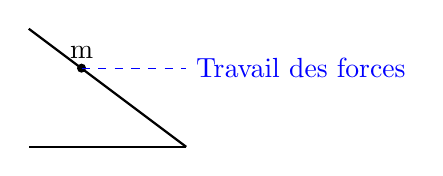
\begin{tikzpicture}
	\draw[thick] (0, 0) -- (-2, 1.5);
	\draw[thick] (0, 0) -- (-2, 0);
	\draw[fill=black] (-1.33, 1) circle (0.05) node [above] {m};
	\draw[dashed, thin, blue] (-1.33, 1) -- (0, 1) node [right] {Travail des forces};
\end{tikzpicture}
\end{wrapfigure}

Dans un système mécanique, on a 2 formes d'énergies : 
\begin{itemize}
	\item une énergie communiquée par $\vec{v}$ dîtes cinétique (qui peut être conservé s'il n'y a pas d'intéraction avec le système) noté $E_c$.
	\item Le travail des forces qui s'appliquent sur \ul{m} noté $E_p$.
\end{itemize}

\paragraph{Exemple}

Ressort de raideur k.

\begin{wrapfigure}[7]{r}{0pt}
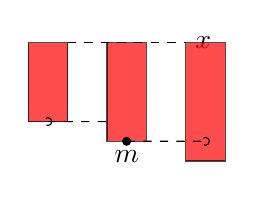
\begin{tikzpicture}
	\draw[fill=red, opacity=0.7] (0, 0) rectangle (0.5, -1);
	\draw[dashed] (0.5, 0) -- (2, 0) node [right] {$x$};
	\draw[fill=red, opacity=0.7] (1, 0) rectangle (1.5, -1.25);
	\draw[fill=red, opacity=0.7] (2, 0) rectangle (2.5, -1.5);
	\draw[dashed] (0.25, -1) circle (0.05) -- (1, -1);
	\draw[dashed] (1.25, -1.25) -- (2.25, -1.25) circle (0.05);
	\draw[fill=black] (1.25, -1.25) circle (0.05) node [below] {$m$};
\end{tikzpicture}
\end{wrapfigure}

PFD : \[
	\begin{array}{rclr}
		m\ddot{x} + kx &=& 0\\
		m(\dot{x}\cdot \ddot{x}) + k\dot{x}x &=& 0  & \text{ Multiplication par } \dot{x} \\
		m \frac{1}{2} \cdot \frac{d}{dt}[(x)]^2 + \frac{1}{2}k\frac{d}{dt}[(x)^2] &=& 0 & \text{ Expression sous forme de derive}\\
		\frac{d}{dt}[(\frac{1}{2}m\dot{x}^2 + \frac{1}{2}kx^2 &=& 0
\end{array}\]

On écrit $\frac{1}{2}m\dot{x}^2 + \frac{1}{2}kx^2 = E_m = \text{ constante }$.

\[
	\begin{array}{rcl}
		{[m\dot{x}^2]} &=& M\cdot(LT^{-1})^2 \\
							  &=& ML^2T^{-2} \\
		{[kx^2]} &=& ML^2T^{-2}
	\end{array}
\]

\begin{itemize}
	\item $\frac{1}{2}m\dot{x}^2$ est l'énergie cinétique. Elle est maximum quand $\frac{1}{2}kx^2 = 0$
	\item $\frac{1}{2}kx^2$ est l'énergie potentielle élastique (conservative) du ressort emmagasinée dans $\Delta x$. La force de rappel du ressort est une force \ul{conservative}
\end{itemize}

Dans un fluide visqueux ($\lambda$) : PFD\[
	\begin{array}{rclr}
		m\ddot{x} + \lambda \dot{x} + kx &=& 0 & \text{ multiplication par} \dot{x} \text{ et écriture sous forme de dérivé} \\
		\frac{d}{dt}[\frac{1}{2}m\dot{x}^2 + \frac{1}{2}kx^2] &=& -\lambda \dot{x}^2 \\
		\frac{d}{dt}E_m &=& \underbrace{-\lambda\dot{x}^2}_{\text{terme dissipatif}} & \text{ theoreme d'Energie mecanique }
	\end{array}
\]
\[
	\left\{
		\begin{array}{c}
			\lambda > 0 \\
			\dot{x} > 0
	\end{array}\right.\]

	Contrairement à $E_p$, $-\lambda \dot{x}^2$ est une force de frottement qui n'est pas conservative.

\section{Travail d'une force}

\begin{wrapfigure}[6]{r}{0pt}
	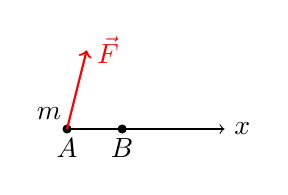
\begin{tikzpicture}

		\draw[fill=black] (0, 0) circle (0.05) node [below]{$A$};
		\node[above left] at (0.05, 0) {$m$};
		\draw[fill=black] (0.7, 0) circle (0.05) node [below]{$B$};
		\draw[->] (0, 0) -- (2, 0) node [right]{$x$};
		\draw[red, thick, ->] (0, 0) -- (0.25, 1) node [right] {$\vec{F}$};
	\end{tikzpicture}
\end{wrapfigure}

$\vec{F}$ : Une force aggissant sur $m$ se déplaçant suivant $Ox$

\paragraph{Définition} Le travail d'une force $\vec{F}$ est défini par : $W_{A \rightarrow B} = \vec{F}\cdot\overrightarrow{AB}$
\paragraph{Remarque} : $W_{B \rightarrow A} = \vec{F}\cdot\overrightarrow{BA} = -W_{A \rightarrow B} $

Pour une force $\vec{F}$ \ul{quelconque} (variable en fonction de la position). On divise l'intervalle $\vec{AB}$ en $N$ sous intervalles sur lesqueles $\vec{F}$ est constante.

\[
	\begin{array}{rcl}
		\vec{F}\overrightarrow{AB} &=& \sum_N(\vec{f}(x) \cdot \frac{\overrightarrow{AB}}{N} \\
								   &=& \vec{F}(x) \sum_{l=1}^{N}(\delta x_l \vec{i}) \\
		\delta x &=& \frac{||\overrightarrow{AB}||}{N} \\
		W_{A \rightarrow B} &=& \sum_{l=1}^N \delta W_l \\
		W_{AB} &=& \lim_{\delta x \to dx} \sum_{l=1}^N dW_l \\
		W_{AB} &=& \int_A^B \vec{F}(x)\cdot dx\vec{i}
\end{array}\]

\paragraph{Travail d'une force}

\[\begin{array}{rcl}
		\text{ Sur 3 dimensions : }	W_{AB} &=& \int_A^B\vec{F}(x, y, z) \cdot (dx\vec{i}+dy\vec{j}+dz\vec{k}) \\
		dW &=& \vec{F}\cdot d\vec{r}
\end{array}\]

\paragraph{Remarque}
\[\begin{array}{rcl}
		{[W]} &=& {[Energie]} \\
			   &=& ML^2T^{-2}\end{array}\]

\begin{itemize}
	\item Si $W_{AB} > 0$, il y a apport d'énergie au système.
	\item Si $W_{AB} < 0$, il y a dissipation d'énergie.
\end{itemize}

\paragraph{Exemples de travail}

$\vec{F} = -kx\cdot \vec{i}$ sur un chemin $A \rightarrow B$.

\[\begin{array}{rcl}
		W_{A\to B}(\vec{F}) &=& \int_A^B(-kx)\vec{i} \cdot (dx\vec{i}) \\
							 &=& \int_A^B(-kxdx) \\
							&=& [-\frac{1}{2}kx^2]^B_A \\
							&=& -[\frac{1}{2}kx^2_B - \frac{1}{2}kx_A]^2 \\
				   &=& \frac{1}{2}k[x_A^2 - x^2_B]
\end{array}\]

\paragraph{Remarque} Le travail d'une force conservatrice ne dépend \ul{Pas} du chemin suivi (Ici il dépend du point de départ, et du point d'arrivé).

\section{Théorème de l'énergie cinétique} La variation de l'énergie cinétique d'un système entre 2 points A et B est égale à la somme des travaux des forces appliquées entre ces points.
\[E_c(B) - E_c(A) = \sum_{\vec{F}} (W_{A \to B}(\vec{F}))\]
